\section{Method}

There are two types of errors that can occur in image segmentation problems.
The first, called a split error, occurs when there are two segments that should have been merged.
The second, called a merge error, happens when one segment should be split into two.
Generally, it is much more difficult to correct merge errors than to correct split errors (CITE). 
Our method takes as input an oversegmentation of an $EM$ image volume where there are many more split errors than merge errors.
Our goal is to identify locations of split errors and merge the corresponding segments.
Section~\ref{sec:neuroproof} discusses two pipelines for generating these segmentations.

From the input segmentation we generate a graph $G$ with nodes $N$ and edges $E$ with weights $w_e$. 
The nodes correspond to label segments from the segmentation with edges between segments considered for merging.
Ideally, our graph has edges corresponding to all of the segments which were erroneously split with few edges between correctly split segments.
We generate a skeleton for every segment following the intuition that a skeleton represents a simplified representation of the overall shape of an object. 
We locate merge candidates and produce corresponding edges based on these skeletons.
A CNN generates the edge weights by learning a merge function given two segments as input. 
A multicut heuristic generates a partition on the graph where nodes in the same partition are assigned the same output label. 
Thus there are three major components to our framework: skeletonization for constructing a graph, network training for determining edge weights, and graph-partitioning using a multicut heuristic algorithm. (INSERT FIGURE HERE)

\subsection{Graph Creation}

We generate nodes $N$ and edges $E$ to apply a graph-based optimization strategy for segmentation. 
In addition, these edges need non-negative weights.

\subsubsection{Node Generation}

The simplest node generation strategy creates one node for every unique segment label in the input volume.
However, some of the millions of labels in the volume correspond to very small regions. 
Usually these locations have noisy image data so the voxel-based methods could not provide enough information to generate a larger segment.
It is difficult to extract useful shape features from these segments because of their small, and often random, shape. 
We prune these nodes from the graph by removing all segments with fewer than $20,000$ voxels. 
On a typical connectomics dataset this only remove XX$\%$ of segments. 

\subsubsection{Edge Generation}

\begin{figure}[t!]
	\centering
	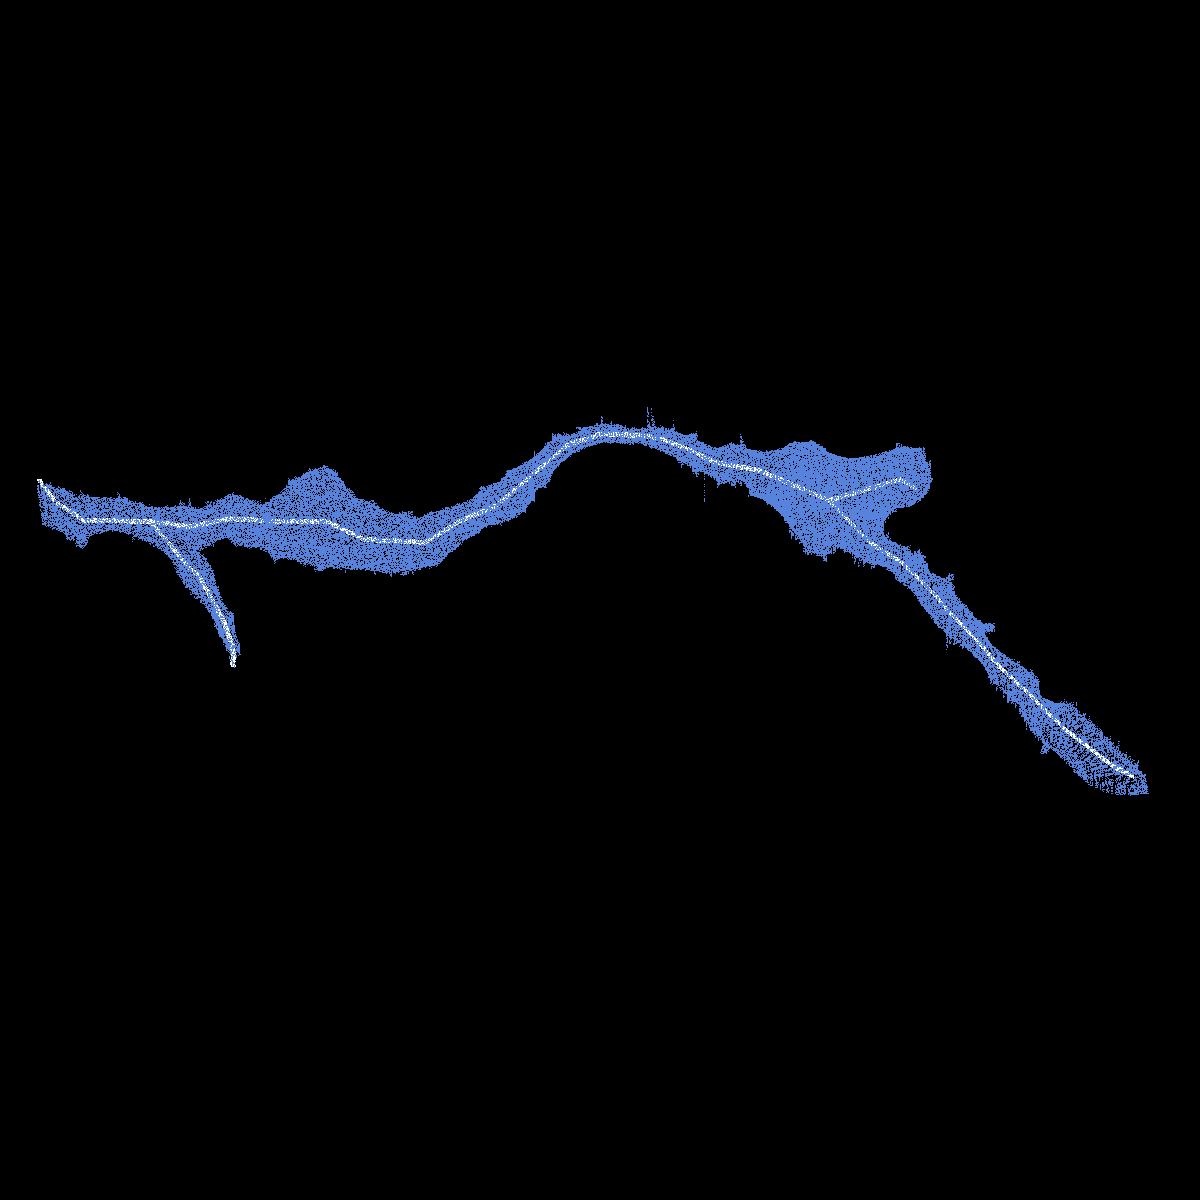
\includegraphics[width=0.42\linewidth]{./figures/skeleton1.png}
	\hspace{0.085\linewidth}
	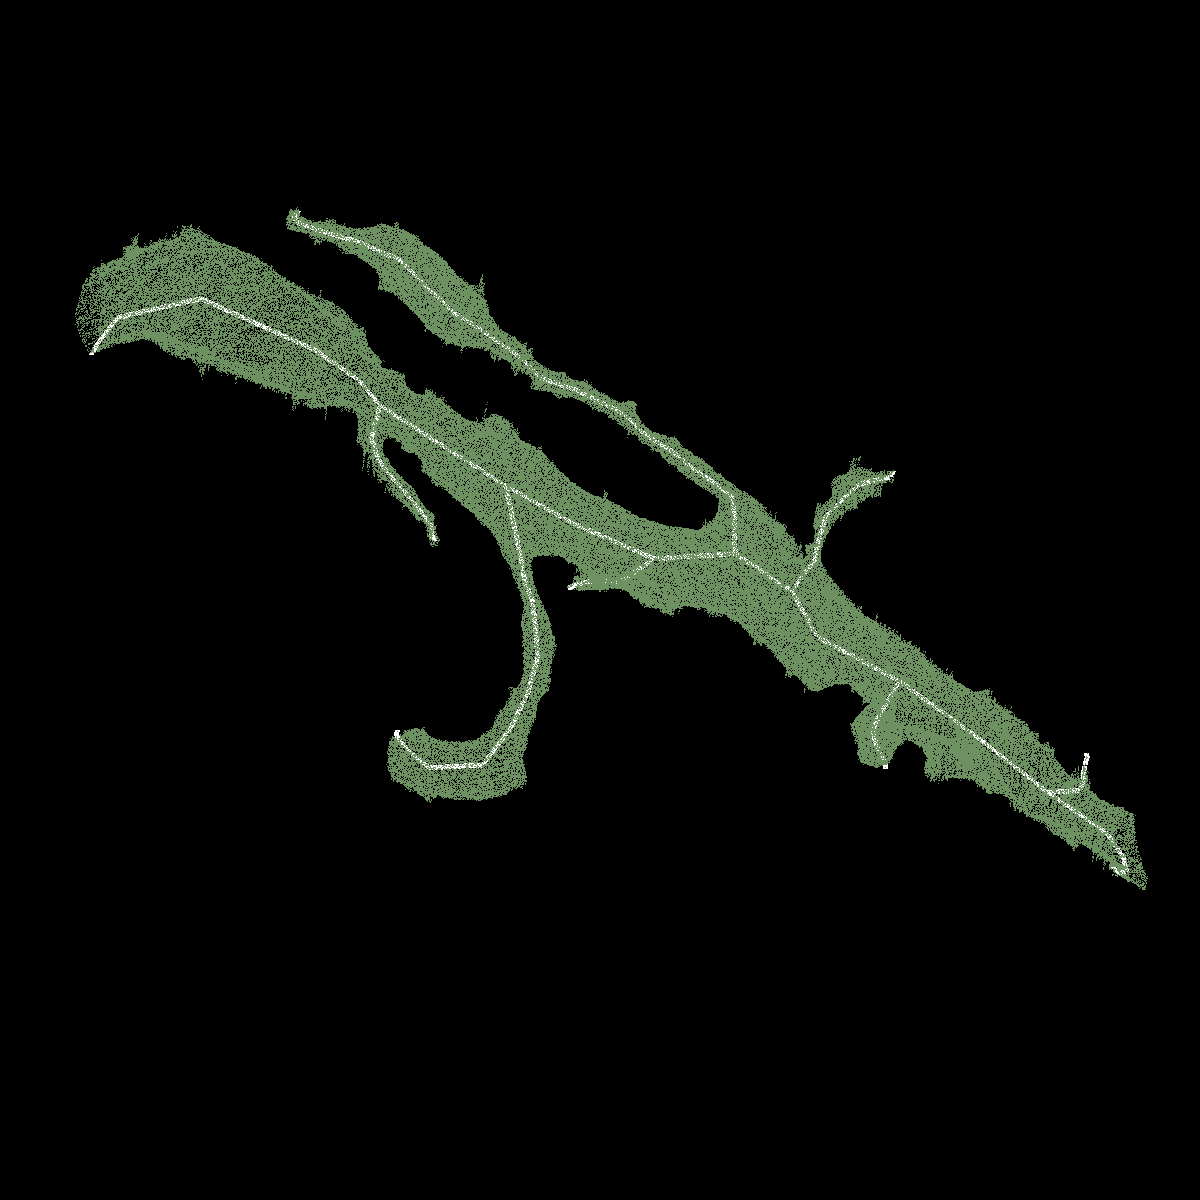
\includegraphics[width=0.42\linewidth]{./figures/skeleton2.png}
	\caption{Two example outputs of the TEASER skeletonization algorithm.}
	\label{fig:skeletonization}
\end{figure}

A na\"ive approach to generating edges produces an edge between all adjacent segments.
Two segments $l_1$ and $l_2$ are considered adjacent if there is a pair of adjacent voxels where one has label $l_1$ and the other has label $l_2$. 
NeuroProof and GALA consider all pairs of adjacent segments for merging. 
This method produces too many edges in the graph for us.
Therefore we present the following algorithm to identify pairs of segments to consider merging. 

First, we extract a skeleton from each segment using the TEASER algorithm~\cite{sato2000teasar,zhao2014automatic}.
Figure~\ref{fig:skeletonization} shows the skeletons in white of two segments from the label volume.
These skeletons consist of a sequence of \textit{joints}, locations that are a local maximum distance from the segment boundary, with line segments connecting successive joints. 
We prune the joints that are within $50$ voxels of each other to reduce unnecessary branching.
For the purposes of our algorithm, joints that have only one connected neighbor are referred to as \textit{endpoints}. 
Many of the segments that are erroneously split follow a similar pattern (Figure~\ref{fig:merge_candidates}). 
In these split instances the skeletons have nearby endpoints.

After skeletonization, we begin to identify segments for merge consideration with the following two-pass heuristic.
In the first pass, we iterate over all endpoints $e$ belonging to a segment $S$ and create a set of segments $\mathbb{S}_e^\prime$ that includes all labels that have a single voxel within $t_{low}$ voxels from $e$. 
Elements of these sets are candidates for merging.
However the first pass often has too many candidates that should remain split so we apply an additional pass for further pruning.
In the second pass, we consider all of the segments $\mathbb{S}_e^\prime$ for every endpoint $e$. 
If a segment $S^\prime \in \mathbb{S}_e^\prime$ has an endpoint within $t_{high}$ voxels of $e$, the segment $S$ and $S^\prime$ are considered for merging. 
We store the midpoint between the two endpoints as the ``center" of the potential merge.
Algorithm (ADD REF) provides pseudocode for this edge generation algorithm. 

\begin{figure}[t]
	\centering
	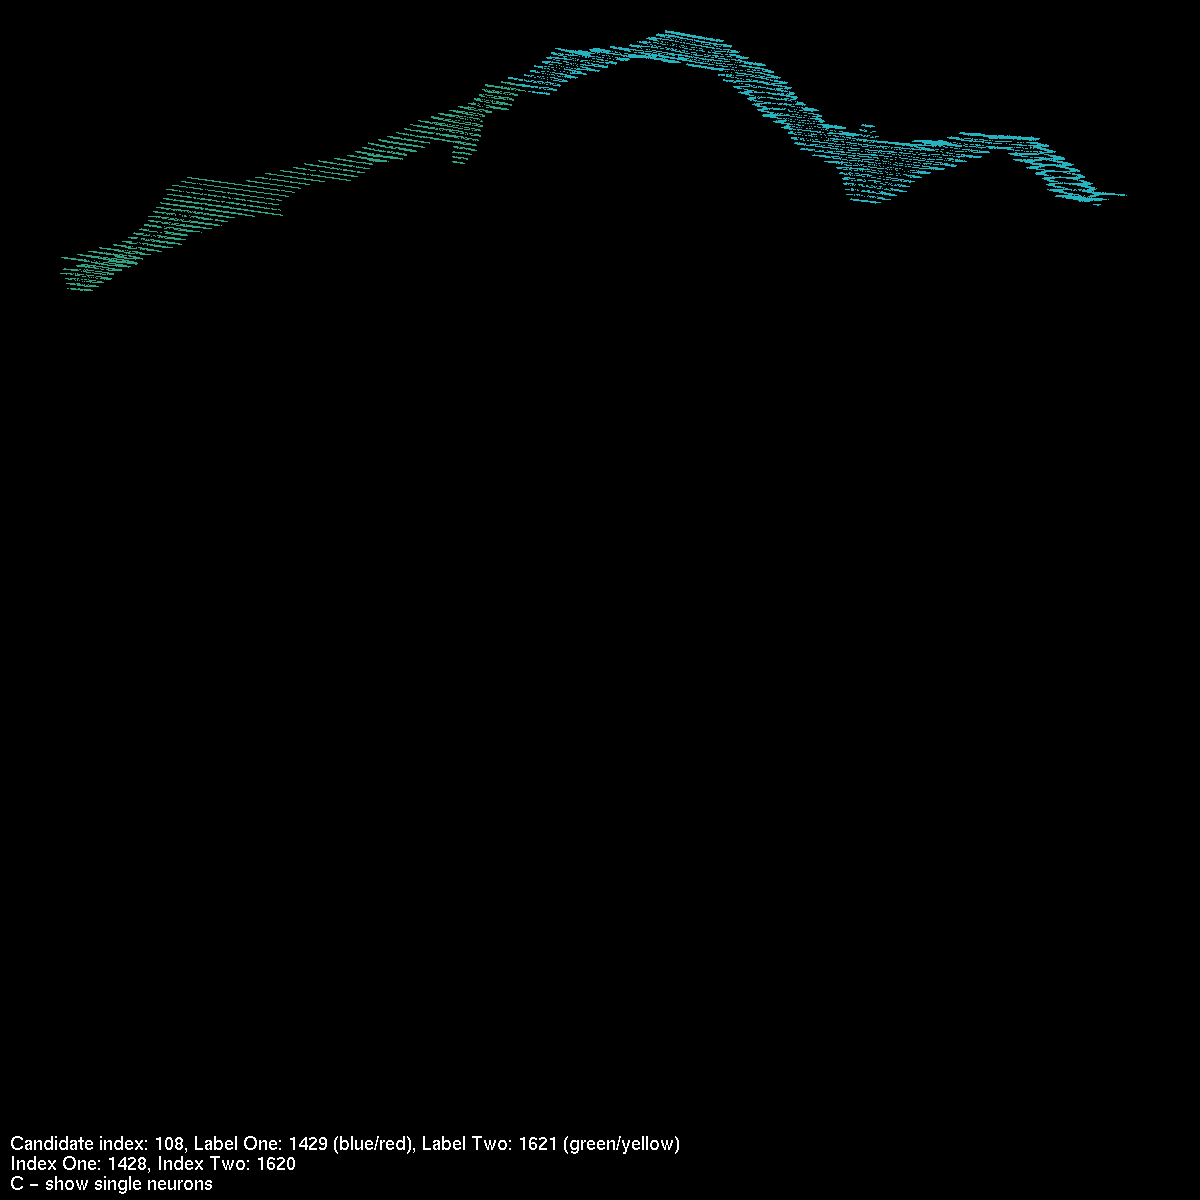
\includegraphics[width=0.42\linewidth]{./figures/split_error1.png}
	\hspace{0.085\linewidth}
	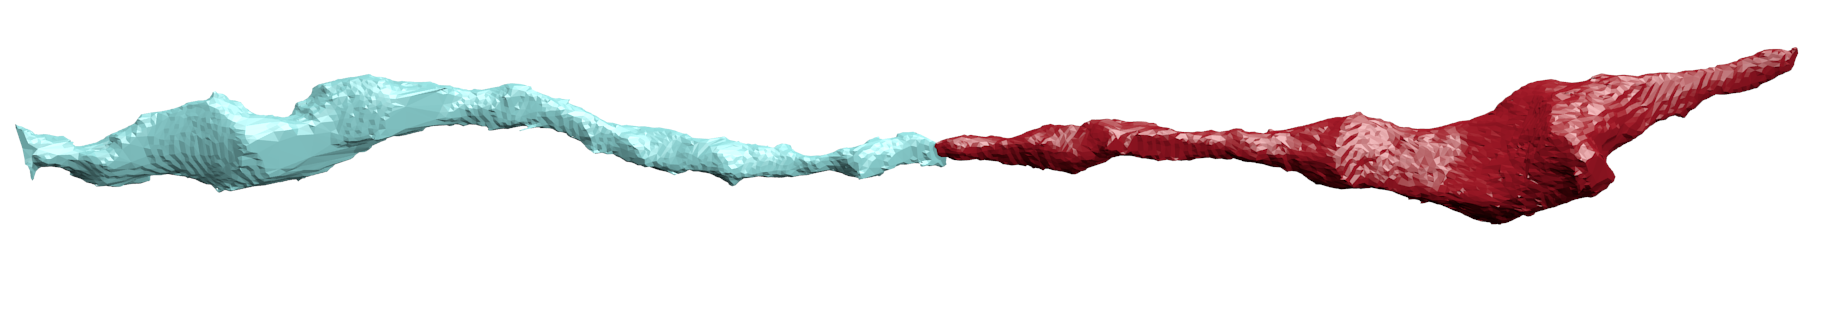
\includegraphics[width=0.42\linewidth]{./figures/split_error2.png}
	\caption{Two erroneously split segments that should merge together. Most segments that we want to merge have the same general structure.}
	\label{fig:merge_candidates}
\end{figure}


\begin{algorithmic}
	\Function{GenerateEdges}{$skeletons$}
		\For {$skeleton$ in $skeletons$}
			\State $candidates$ = set()
			\For {$endpoint$ in $skeleton$}
				\State TODO ADD CODE
			\EndFor
		\EndFor
	\EndFunction
\end{algorithmic}

Note that this algorithm does not enforce any segment adjacency constraints.
Figure (ADD FIGURE) shows two examples that would not be considered in NeuroProof or GALA since these algorithms only consider merging adjacent segments.

\subsection{Edge Probabilities}

The previous section outlines how to generate edges between nodes in our graph structure. 
Here we introduce a neural network architecture for generating probabilities that two nodes sharing an edge belong to the same neuron. 
The neural network takes as input only data from the input segmentation. 

\subsubsection{Network Architecture}

Our graph generation algorithm produces 3-D locations that require further consideration for merging. 
To determine which of these segments should actually merge, we train a 3-D CNN using the oversegmentation and the corresponding manually labeled ground truth data (Section~\ref{sec:dataset}).
We extract a cubic region of interest around these locations as input to the CNN. 
These regions of interests will provide the local information for the neural network to predict which neighboring segments belong to the same neuron. 

The networks receives three input channels for every voxel in the region of interest around segments $l_1$ and $l_2$. 
The input to all of the channels is in the set $\{-0.5, 0.5\}$. 
The first channel is $0.5$ only if the corresponding voxel has label $l_1$. 
The second channel is $0.5$ only if the corresponding voxel has label $l_2$. 
The third channel is $0.5$ if the corresponding voxel is either $l_1$ or $l_2$. 

Figure~\ref{fig:architecture} provides an overview of our architecture. 
Our network architecture has three layers of double convolutions followed by a max pooling step following the work of Chatfield et al. that found such a framework improves on single convolution layers~\cite{chatfield2014return}. The first two max pooling layers are anisotropic with pooling only in the $x$ and $y$ dimensions to account for the anisotropic nature of the datasets.
The output after this final pooling step is flattened into a 1-D vector which is input into two fully connected layers.
The final layer produces a probability with a sigmoid activation function~\cite{funahashi1989approximate}. 
All of the other activation functions are LeakyReLU~\cite{maas2013rectifier}. 
We use a stochastic gradient descent optimizer with Nesterov's accelerated gradient~\cite{nesterov1983method}. 
There are dropouts of $0.2$ after every pooling layer and the first dense layer, and a dropout of $0.5$ after the final dense layer. 
This prevents overfitting of the training data.


\begin{figure*}[t]
	\centering
	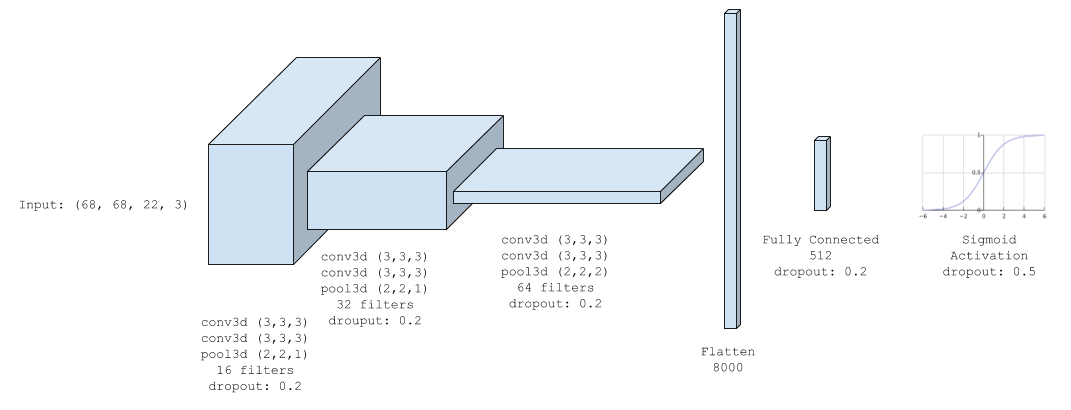
\includegraphics[width=0.95\linewidth]{figures/architecture.png}
	\caption{The architecture for the neural networks follows the \textit{VGG} style of double convolutions followed by a max pooling operation. The number of filters doubles each layer leading to a fully connected layer and a sigmoid activation function.}
	\label{fig:architecture}
\end{figure*}

\subsection{Agglomeration}

After constructing the graph structure we apply a graph-based segmentation strategy. 
There are many formulations of graph-based optimization strategies that provide different guarantees on their output. 
Neurons in the brain should be acyclic, i.e. the output shape should have a genus of zero. 
Current connectomics agglomeration techniques do not leverage this additional information but rather consider neighboring regions in successive order without regard to loop creation. 
In our graph formulation we enforce this topological property by applying a multicut partition onto the graph that generates a \textit{forest} on the nodes. 
A forest is a partitioning of a graph into a set of trees (i.e. no segment has a cycle). 
There are several heuristics that solve the multicut problem. For our purposes we use the Kernighan-Lin algorithm~\cite{kernighan1970efficient}.
The running time of this algorithm is $\mathcal{O}(N^3)$, where $N$ is the number of nodes in the graph (DOUBLE CHECK). 